\documentclass{beamer}
\usepackage{hyperref}
\usepackage[T1]{fontenc}
\usepackage{media9}

\hypersetup{
    colorlinks=true,
    linkcolor=magenta,     
    urlcolor=blue,
    pdfpagemode=FullScreen,
}

% other packages
\usepackage{latexsym,amsmath,xcolor,multicol,booktabs,calligra}
\usepackage{graphicx,pstricks,listings,stackengine}

\author{Pradyumnan R}
\title{Understanding DSMC, SPARTA and results from simulating 1D Fourier flow using SPARTA}
%\subtitle{}
\institute{JNCASR}
\date{July 2, 2024}
\usepackage{USTC_beamer}

% \renewcommand{\familydefault}{\rmdefault}

%%%%%%%%%%%%%%%%%%%%%%%%%%%%%%%%%% My own packages  %%%%%%%%%%%%%%%%%%%%%%%%%%%%%%%%%%%
\usepackage{svg}
\usepackage{caption}
\captionsetup{font=footnotesize}

% defs
\def\cmd#1{\texttt{\color{red}\footnotesize $\backslash$#1}}
\def\env#1{\texttt{\color{blue}\footnotesize #1}}
\definecolor{deepblue}{rgb}{0,0,0.5}
\definecolor{deepred}{rgb}{0.6,0,0}
\definecolor{deepgreen}{rgb}{0,0.5,0}
\definecolor{halfgray}{gray}{0.55}

\lstset{
    basicstyle=\ttfamily\small,
    keywordstyle=\bfseries\color{deepblue},
    emphstyle=\ttfamily\color{deepred},    % Custom highlighting style
    stringstyle=\color{deepgreen},
    numbers=left,
    numberstyle=\small\color{halfgray},
    rulesepcolor=\color{red!20!green!20!blue!20},
    frame=shadowbox,
}

\begin{document}

% \kaishu
\renewcommand{\figurename}{Fig.} % Comment this out you will have “图1”

% logo
\begin{frame}
    \titlepage
    \begin{figure}[htpb]
        \begin{center}
            
\includegraphics[width=0.2\linewidth]{Pictures/JNCASR_Logo.png}
        \end{center}
    \end{figure}
\end{frame}

\begin{frame}                       
    \tableofcontents[sectionstyle=show,subsectionstyle=show/shaded/hide,subsubsectionstyle=show/shaded/hide]
    
\end{frame}

\section{Direct Simulation Monte Carlo}

    \subsection{General information}

        \begin{frame}{General Information}
            \begin{itemize}
                \setlength\itemsep{0.25cm}
                
                \item<1->The DSMC method is used whenever the Knudsen number is of the order of 1. For example, it is used in MEMS and Space Shuttle re-entry aerodynamics
    
                \item<2->It models fluid flows using probabilistic simulation molecules to solve the Boltzmann equation
    
                \item<3-> DSMC is better at describing the non-equilibrium behaviour of gases than most continuum models such as Navier-Stokes through higher fidelity\cite{plimpton2019direct}
            \end{itemize}
        \end{frame}

    \subsection{The algorithm}

        \begin{frame}{The algorithm}
            \begin{itemize}
                \setlength\itemsep{0.25cm}
                
                \item<1->The state of a system is given by the positions and velocities of the particles $\{ \vec{r_i}, \vec{v_i} \}$ where $i = 1, 2, 3, \cdots, N$ and $N$ is the number of particles

                \item<2->Each DSMC particle represents $F_N$ particles in physical space with approximately the same positions and velocities

                \item<3->The evolution of the system is integrated in time steps $\tau$ lesser than the mean collision time

                \item<4->Without external forces like gravity, the particles are said to move balistically, i.e., $\vec{r}_i(t + \tau) = \vec{r}_i(t) + \vec{v}_i(t)\tau$

                \item<5->If a particle reaches a boundary, it's position and velocity are reset accordingly
            \end{itemize}
        \end{frame}

        \begin{frame}{The algorithm (boundary collisions)}
            \begin{columns}
                \begin{column}{0.5\linewidth}
                    \begin{figure}
                        \centering
                        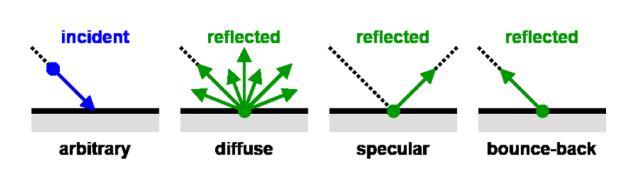
\includegraphics[width=\linewidth]{Pictures/Literature/Bound_Refl.png}
                        \caption{Various types of boundary collisions}
                        \label{Grid}
                    \end{figure}
                \end{column}
        
                \begin{column}{0.5\linewidth}
                    \begin{itemize}
                        \setlength\itemsep{0.25cm}
                        
                        \item<1->The specular boundary collision is simply the preservance of the angle between the normal and the particle trajectory just before and after collision
                
                        \item<2->Diffuse boundary collisions are when there is a degree of randomness ($\alpha$) in the specularity of the collision
                    \end{itemize}
                \end{column}
            \end{columns}
        \end{frame}

        \begin{frame}{The algorithm}
            \begin{itemize}
                \setlength\itemsep{0.25cm}
                
                \item<1->After all particles are moved, they are put into cells within which they randomly collide based on collision rates and probabilities obtained from the kinetic theory of gases

                \item<2->The dimension of each collision cell is no longer than a mean free path. All particles in a cell are collision candidates, regardless of their actual trajectories

                \item<3->For the \textbf{hard spheres} collision model, the collision probability for the pair of particles $i$ and $j$ is proportional to their relative speed,
                
                    \begin{equation*}
                        P_{coll}[i, j] = \frac{|\vec{v}_i - \vec{v}_j|}{\sum_{m=1}^{N_c} \sum_{n=1}^{m-1} |\vec{v}_m - \vec{v}_n|}
                    \end{equation*}
                
                $N_c$ is the number of particles in the cell
            \end{itemize}
        \end{frame}

        \begin{frame}{The algorithm}
            \begin{itemize}
                \setlength\itemsep{0.25cm}
                
                \item<1->The double summation in the denominator can be computationally intensive, so a technique called \textbf{rejection sampling} is used to select collision pairs

                    \begin{equation*}
                        v_r > v_{r_{max}} \cdot \mathcal{R} \text{ for } \mathcal{R}\in [0,1]
                    \end{equation*}

                \item<2->The total number of hard sphere collisions given in a cell during a time $` \tau `$ is given by

                    \begin{equation*}
                        M_{coll} = \frac{1}{2} (N_c - 1) F_N f_{coll} \tau = \frac{N_c (N_c - 1) F_N \pi d^2 \langle v_r \rangle \tau}{2 V_c}
                    \end{equation*}

                where $f_{coll}$ is the collision frequency given by KTG, $d$ is the diameter of the cell and $V_c$ is the volume of the cell
            \end{itemize}
        \end{frame}

\section{Existing Literature}

    \subsection{DSMC on petaflop supercomputers and beyond \cite{plimpton2019direct}}

        \begin{frame}{SPARTA}
            \begin{columns}
                \begin{column}{0.5\linewidth}
                    \begin{figure}
                        \centering
                        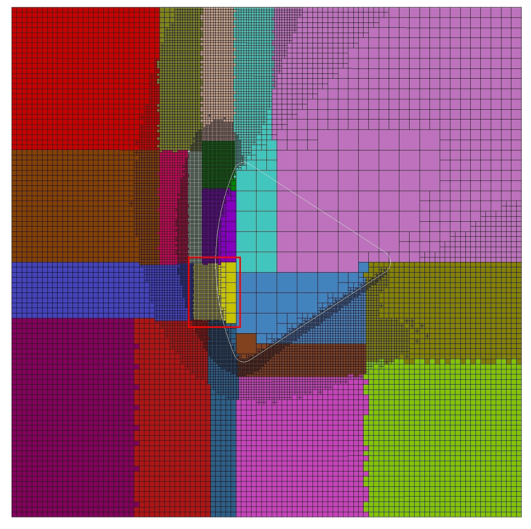
\includegraphics[width=\linewidth]{Pictures/Literature/Grid.png}
                        \caption{Grid Hierarchy in SPARTA}
                        \label{Grid}
                    \end{figure}
                \end{column}
        
                \begin{column}{0.5\linewidth}
                    \begin{itemize}
                        \setlength\itemsep{0.25cm}
                        
                        \item<1-> DSMC is inherently parallel. It has three kinds of elements : particles, grid cells and surfaces
                
                        \item<2-> Grid cells are indexed hierarchically using bits. Cells store information about everything within them
    
                        \item<3-> Each processor owns \textbf{ghost cells} that extend beyond its domain to minimize MPI calls during the run
                    \end{itemize}
                \end{column}
            \end{columns}
        \end{frame}
    
        \begin{frame}{SPARTA}
            \begin{columns}
                \begin{column}{0.5\linewidth}
                    \begin{figure}
                        \centering
                        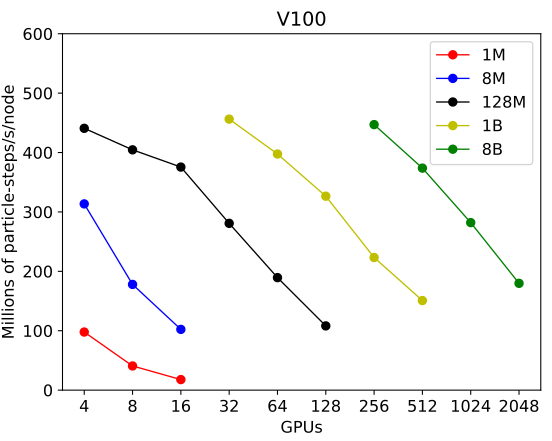
\includegraphics[width=\linewidth]{Pictures/Literature/GPU.png}
                        \caption{GPU Parallelisation in SPARTA}
                        \label{gra:GPU}
                    \end{figure}
                \end{column}
        
                \begin{column}{0.5\linewidth}
                    \begin{itemize}
                        \setlength\itemsep{0.25cm}
                        
                        \item<1-> A typical simulation has about 20 particles per grid cell for adequate collision statistics
    
                        \item<2-> GPU parallelisation is seen to be more efficient for larger problems (Figure \ref{gra:GPU})
                        
                        \item<3-> Performance per GPU decreases but the aggregate performance increases
                    \end{itemize}
                \end{column}
            \end{columns}
        \end{frame}

    \subsection{Effect of slip on vortex shedding from a circular cylinder in a gas flow \cite{gallis2021effect}}

        \begin{frame}{Key Takeaways}
            \begin{columns}
                \begin{column}{0.5\linewidth}
                    \begin{itemize}
                        \setlength\itemsep{0.25cm}
                                
                        \item<1->The relation between Knudsen number, Mach number and Reynold's number for gases is given by
        
                            \begin{equation*}
                                Kn = \frac{Ma}{Re} \sqrt{\frac{\gamma \pi}{2}}
                            \end{equation*}
        
                        \item<2-> The simulation given in Figure \ref{img:Vortex} was simulated using both DSMC and COMSOL Multiphysics
                    \end{itemize}                    
                \end{column} 
            
                \begin{column}{0.5\linewidth}
                    \begin{figure}
                        \centering
                        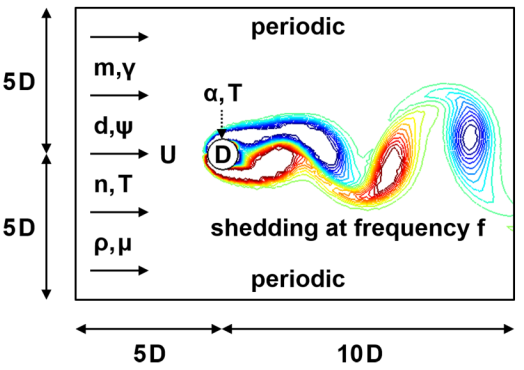
\includegraphics[width=\linewidth]{Pictures/Literature/Vortex_Shedding.png}
                        \caption{Vortex Shedding Setup}
                        \label{img:Vortex}
                    \end{figure}
                \end{column}
            \end{columns}
        \end{frame}
        
        \begin{frame}{Boundary Conditions}
            \begin{columns}
                \begin{column}{0.5\linewidth}
                    \begin{itemize}
                        \setlength\itemsep{0.25cm}
                                
                        \item<1-> The outlet boundary conditions by DSMC are the \textbf{inlet boundary condition} (Figure \ref{img:Outlet} img whereas CFD applies zero pressure and zero viscous stress	
                        
                        \item<2-> The inlet is at Ma = 0.3, Re = 100 and Kn = 0.0048
                    \end{itemize}                    
                \end{column} 
            
                \begin{column}{0.5\linewidth}
                    \begin{figure}
                        \centering
                        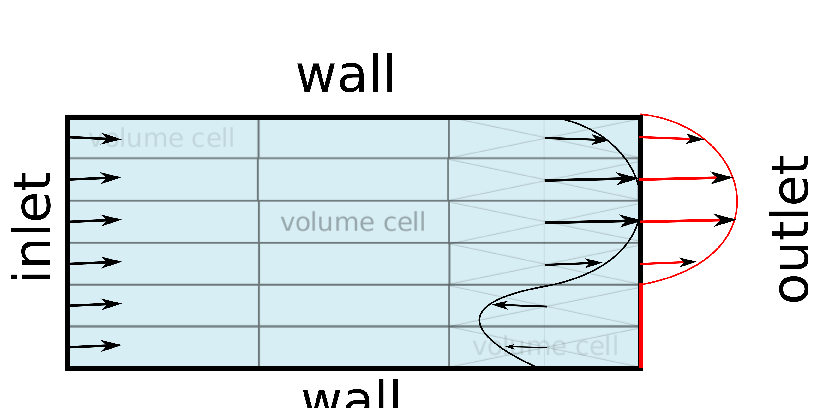
\includegraphics[width=\linewidth]{Pictures/Literature/Outlet.png}
                        \caption{Inlet boundary conditions at outlet}
                        \label{img:Outlet}
                    \end{figure}
                \end{column}
            \end{columns}
        \end{frame}

        \begin{frame}{Comparing Results from DSMC and CFD}
            \begin{figure}
                \centering
                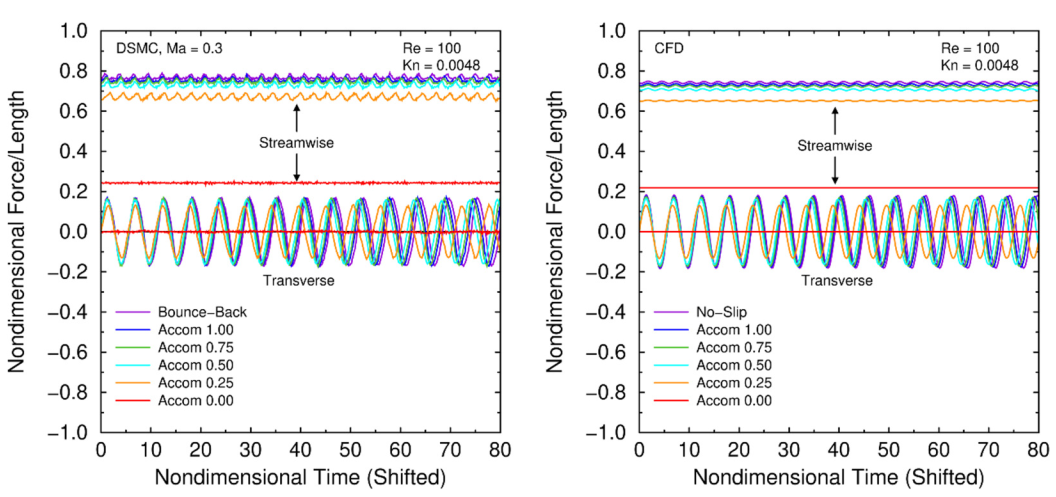
\includegraphics[width=0.7\linewidth]{Pictures/Literature/Compare.png}
                \caption{Left : DSMC and Right : CFD}
                \label{gra:Comp}
            \end{figure}

            \begin{itemize}
                \setlength\itemsep{0.25cm}
                                
                \item<1->Figure \ref{gra:Comp} illustrates the agreement between DSMC and CFD.

                \item<2-> As the Reynold's number decreases, the slip increases.
            \end{itemize}
        \end{frame}

\section{1D Fourier Flow using SPARTA}

    \subsection{Knudsen number fixed at 0.1}

        \begin{frame}{The problem and the simulation details}
            \begin{columns}
                \begin{column}{0.5\linewidth}
                    \begin{itemize}
                        \setlength\itemsep{0.25cm}
                                
                        \item<1->The setup of the simulation is given by Figure \ref{img:Setup}. The gas used is Argon

                        \item<2->The simulation parameters are given below \cite{rader2005dsmc}

                            \begin{equation*}
                                \lambda = 10^{-4} m \hspace{1cm} \Delta t = 10^{-8} s
                            \end{equation*}

                            \begin{equation*}
                                N = 1.682 \times 10^{14} \hspace{1cm} t_o = 71 ns
                            \end{equation*}
                    \end{itemize}                    
                \end{column} 
            
                \begin{column}{0.5\linewidth}
                    \begin{figure}
                        \centering
                        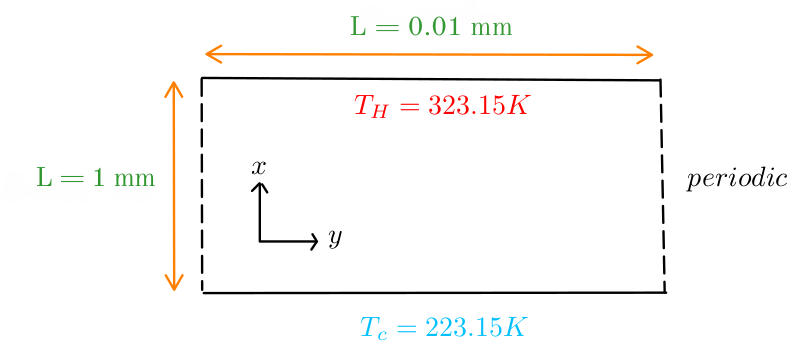
\includegraphics[width=\linewidth]{Pictures/1D_Fourier_Flow/Setup.png}
                        \caption{Simulation Setup}
                        \label{img:Setup}
                    \end{figure}
                \end{column}
            \end{columns}
        \end{frame}

        \begin{frame}{The results at 20 particles per grid cell}
            \begin{columns}
                \begin{column}{0.5\linewidth}
                    \begin{itemize}
                        \setlength\itemsep{0.25cm}
                                
                        \item<1->The temperature profile in Figure \ref{gra:kn0.1_20ppgc_100g} clearly resembling a linear profile

                        \item<2-> A clear distinction can be seen from the expected continuum solution due to rarefraction effects
                    \end{itemize}                    
                \end{column} 
            
                \begin{column}{0.5\linewidth}
                    \begin{figure}
                        \centering
                        \includesvg[width=\linewidth]{Pictures/1D_Fourier_Flow/Temperature_0.010000_sec_20ppgc}
                        \caption{}
                        \label{gra:kn0.1_20ppgc_100g}
                    \end{figure}
                \end{column}
            \end{columns}
        \end{frame}

        \begin{frame}{The results at 100 particles per grid cell}
            \begin{columns}
                \begin{column}{0.5\linewidth}
                    \begin{itemize}
                        \setlength\itemsep{0.25cm}
                                
                        \item<1->The temperature profile in Figure \ref{gra:kn0.1_100ppgc_100g} clearly resembling a linear profile

                        \item<2-> A clear distinction can still be seen from the expected continuum solution due to rarefraction effects

                        \item<3-> However the statistical fluctuations are much less pronounced
                    \end{itemize}                    
                \end{column} 
            
                \begin{column}{0.5\linewidth}
                    \begin{figure}
                        \centering
                        \includesvg[width=\linewidth]{Pictures/1D_Fourier_Flow/Temperature_0.010000_sec_100ppgc.svg}
                        \caption{}
                        \label{gra:kn0.1_100ppgc_100g}
                    \end{figure}
                \end{column}
            \end{columns}
        \end{frame}

        \begin{frame}{The results at 100 particles per grid cell but with twice the resolution}
            \begin{columns}
                \begin{column}{0.5\linewidth}
                    \begin{itemize}
                        \setlength\itemsep{0.25cm}
                                
                        \item<1->The temperature profile in Figure \ref{gra:kn0.1_100ppgc_200g} clearly resembling a linear profile

                        \item<2-> A clear distinction can still be seen from the expected continuum solution due to rarefraction effects

                        \item<3-> The deviation from the analytical solution doesn't reduce by resolving the grid. We can safely infer that the deviation is not a numerical error
                    \end{itemize}                    
                \end{column} 
            
                \begin{column}{0.5\linewidth}
                    \begin{figure}
                        \centering
                        \includesvg[width=\linewidth]{Pictures/1D_Fourier_Flow/Temperature_0.010000_sec_200g.svg}
                        \caption{}
                        \label{gra:kn0.1_100ppgc_200g}
                    \end{figure}
                \end{column}
            \end{columns}
        \end{frame}

    \subsection{Knudsen number fixed at 0.02}

        \begin{frame}{The problem and the simulation details}
            \begin{columns}
                \begin{column}{0.5\linewidth}
                    \begin{itemize}
                        \setlength\itemsep{0.25cm}
                                
                        \item<1->The setup of the simulation is given by Figure \ref{img:Setup}. The gas used is Argon

                        \item<2->The simulation parameters are given below \cite{rader2005dsmc}

                            \begin{equation*}
                                \lambda = 10^{-4} m \hspace{1cm} \Delta t = 10^{-8} s
                            \end{equation*}

                            \begin{equation*}
                                N = 8.41 \times 10^{14} \hspace{1cm} t_o = 71 ns
                            \end{equation*}
                    \end{itemize}                    
                \end{column} 
            
                \begin{column}{0.5\linewidth}
                    \begin{figure}
                        \centering
                        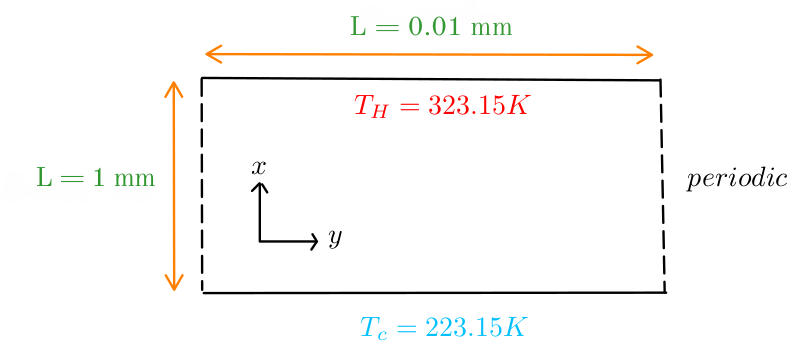
\includegraphics[width=\linewidth]{Pictures/1D_Fourier_Flow/Setup.png}
                        \caption{Simulation Setup}
                        \label{img:Setup}
                    \end{figure}
                \end{column}
            \end{columns}
        \end{frame}

        \begin{frame}{The results at 100 particles per grid cell}
            \begin{columns}
                \begin{column}{0.5\linewidth}
                    \begin{figure}
                        \centering
                        \includesvg[width=\linewidth]{Pictures/1D_Fourier_Flow/Temperature_0.010000_sec_kn0.02.svg}
                        \caption{}
                        \label{gra:kn0.1_100ppgc_kn0.02}
                    \end{figure}
                \end{column}
            
                \begin{column}{0.5\linewidth}
                    \begin{itemize}
                        \setlength\itemsep{0.25cm}
                                
                        \item<1->The temperature profile in Figure \ref{gra:kn0.1_100ppgc_kn0.02} clearly resembling a linear profile

                        \item<2->Here, the simulation closely resembles the analytical solution.

                        \item<3->We can conclude that the closer the Knudsen number is to zero, the simulation will agree more with the analytical solution
                    \end{itemize}                    
                \end{column} 
            \end{columns}
        \end{frame}

	\subsection{Visualising the fluctuations in the solution}
	
		\begin{frame}{Fluctuations as a function of the number of particles per grid cell}
			\begin{itemize}
				\item<1-> Let's visualize the fluctuations of the solution for different number of particles per grid cell using a few videos.
			\end{itemize}
		\end{frame}	       

\section{References}

    \bibliographystyle{plain}
    \bibliography{refs}

\end{document}